% !TEX TS-program = pdflatex
\documentclass[aspectratio=169]{beamer}
\usepackage[utf8]{inputenc}
\usepackage[T1]{fontenc}
\usetheme{Madrid}
\usecolortheme{seahorse}
\usefonttheme{professionalfonts}
\setbeamertemplate{navigation symbols}{}
\setbeamercovered{transparent}
\setbeamertemplate{itemize items}[circle]
\setbeamertemplate{enumerate items}[default]
\setlength{\parskip}{0.15em}

\definecolor{bepurple}{RGB}{107,63,160}
\definecolor{begold}{RGB}{200,168,75}
\definecolor{beteal}{RGB}{26,122,110}
\definecolor{berust}{RGB}{192,68,42}
\definecolor{beblue}{RGB}{26,74,138}
\definecolor{softpurple}{RGB}{240,232,255}
\definecolor{softgold}{RGB}{255,248,220}
\definecolor{softteal}{RGB}{220,242,240}
\definecolor{softrust}{RGB}{255,235,230}
\setbeamercolor{structure}{fg=beblue}
\setbeamercolor{title}{fg=white,bg=beblue}
\setbeamercolor{frametitle}{fg=beblue}
% Minimal block rendering: regular/example blocks become colored headings (no box)
\setbeamertemplate{block begin}{%
  \par\vspace{0.2ex}%
  \ifx\insertblocktitle\empty\else%
    {\usebeamerfont{block title}\color{beblue}\textbf{\insertblocktitle}}\par\vspace{0.2ex}%
  \fi%
}
\setbeamertemplate{block end}{\par\vspace{0.2ex}}
\setbeamertemplate{block example begin}{%
  \par\vspace{0.2ex}%
  \ifx\insertblocktitle\empty\else%
    {\usebeamerfont{block title}\color{beteal}\textbf{\insertblocktitle}}\par\vspace{0.2ex}%
  \fi%
}
\setbeamertemplate{block example end}{\par\vspace{0.2ex}}
\setbeamertemplate{block alerted begin}{%
  \par\vspace{0.5ex}%
  \begin{beamercolorbox}[sep=0.5ex,rounded=true,shadow=false]{block title alerted}%
    \usebeamerfont{block title}\insertblocktitle%
  \end{beamercolorbox}%
  \nointerlineskip%
  \begin{beamercolorbox}[sep=0.5ex,rounded=true,shadow=false]{block body alerted}%
    \usebeamerfont{block body}%
}
\setbeamertemplate{block alerted end}{\end{beamercolorbox}\par\vspace{0.5ex}}
\setbeamercolor{block title alerted}{fg=white,bg=berust}
\setbeamercolor{block body alerted}{fg=black,bg=berust!8}
\setbeamercolor{alerted text}{fg=berust}

\usepackage{booktabs,amsmath,amssymb,array,multirow,hyperref,colortbl,xcolor}
\usepackage{tikz}
\usepackage{pgfplots}
\pgfplotsset{compat=1.18}
\usetikzlibrary{arrows.meta,positioning,calc,shapes.geometric,patterns}
\hypersetup{colorlinks=true,linkcolor=beblue,urlcolor=beblue}

\title{\textbf{Lecture 6: Social Preferences}}
\subtitle{Fairness, Reciprocity, and Why We Are Not Purely Selfish}
\author{Prof.\ Muhebullah Karimzada}
\institute{School of Economics, University of Northern British Columbia}
\date{ECON 230 $\cdot$ Introduction to Behavioural Economics $\cdot$ Winter 2027}

\begin{document}

\begin{frame}[plain]\titlepage\end{frame}

% ============================================================
\begin{frame}{Opening Puzzle --- Would You Reject This?}
\note{The rational self-interest answer is 'yes, accept' -- $5 > 0 always. But about 50\% of people reject offers below 30\%. This is your opening hook.}
\begin{alertblock}{The Ultimatum Game --- Your Decision}
You and a stranger have been given \textbf{\$30} to split. The stranger decides how to split it. You either:
\begin{itemize}
  \item \textbf{Accept}: You get the offered amount; the stranger keeps the rest.
  \item \textbf{Reject}: You both get \textbf{\$0}.
\end{itemize}
\textbf{The stranger offers you \$5. Do you accept?}\\[0.4em]
\textit{(Write your answer. Standard economics says: YES --- \$5 > \$0.)}
\end{alertblock}
\pause
\begin{block}{Typical Result}
In hundreds of experiments worldwide, \textbf{50\% of subjects reject offers below \$3 out of \$10}. They willingly sacrifice their own payoff to punish unfair behaviour. Standard economics cannot explain this. Today we study why.
\end{block}
\end{frame}

% ============================================================
\begin{frame}{Lecture Overview}
\begin{enumerate}[<+->]
  \item \textbf{Why social preferences matter} --- departures from pure self-interest
  \item \textbf{Ultimatum Game} --- costly punishment of unfairness
  \item \textbf{Dictator Game} --- pure giving, no strategic motive
  \item \textbf{Trust Game} --- trust, trustworthiness, and economic growth
  \item \textbf{Fehr-Schmidt Model} --- inequality aversion (envy and guilt)
  \item \textbf{Reciprocity and altruism} --- giving and punishing
  \item \textbf{Public goods games} --- free-riding and altruistic punishment
  \item \textbf{Applications} --- labour markets, wages, corporate responsibility, corruption
\end{enumerate}
\end{frame}

% ============================================================
\section{Pure Self-Interest and Its Failures}
% ============================================================

\begin{frame}{The Standard Assumption and the Evidence Against}
\begin{block}{Standard Economics}
Agents maximise their \textit{own} material payoff. Other people's payoffs enter only if they affect your own (rival goods, externalities).
\end{block}
\begin{center}
\begin{tabular}{lcc}
\toprule
\textbf{Experiment} & \textbf{Nash Prediction} & \textbf{Typical Result}\\
\midrule
Ultimatum Game & Offer \$0.01; Responder accepts & Mean offer $\approx$40\%; 50\% reject $<$20\%\\
Dictator Game & Give \$0 & Mean giving $\approx$28\%\\
Trust Game & Send \$0 & Average sent $\approx$50\%\\
Public Goods & Contribute \$0 & Contribute 40--60\% initially\\
\bottomrule
\end{tabular}
\end{center}
\begin{alertblock}{These Are Not Errors --- They Are Preferences}
The gap between Nash predictions and actual behaviour is \textit{systematic}, \textit{stable}, and \textit{replicable}. People have genuine preferences over others' outcomes. This is \alert{social preferences}.
\end{alertblock}
\end{frame}

% ============================================================
\section{The Ultimatum Game}
% ============================================================

\begin{frame}{[GAME] The Ultimatum Game --- Play Now}
\note{Pair students. One is Proposer, one is Responder. They write offers and acceptance decisions on paper simultaneously. Reveal results. Show the distribution of offers and rejections on the board.}
\begin{block}{Rules}
\begin{enumerate}
  \item Pair up with your neighbour. Decide who is \textbf{Proposer} (P) and who is \textbf{Responder} (R).
  \item P divides a hypothetical \textbf{10 tokens} between P and R. Write the offer to R (0--10).
  \item R does not see P's offer yet. R writes a \textbf{minimum acceptable offer} (0--10).
  \item If P's offer $\geq$ R's minimum: both get the amounts. If P's offer $<$ R's minimum: both get \textbf{0}.
\end{enumerate}
\end{block}
\begin{block}{Data Collection}
Show of hands: What did Proposers offer? What was the lowest accepted offer? Were any offers rejected? \textit{Prof will compile results on the board.}
\end{block}
\begin{exampleblock}{What to Expect}
Modal offer: 4--5 tokens (40--50\%). Rejections: common for offers below 2--3 tokens. Very few offer 0 or 1. Prediction: your class results will mirror the worldwide experimental literature.
\end{exampleblock}
\end{frame}

% ============================================================
\begin{frame}{Ultimatum Game --- Worldwide Data}
\begin{columns}
\column{0.5\textwidth}
\begin{tikzpicture}
\begin{axis}[
  width=\textwidth,height=0.55\textheight,
  xlabel={\small Offer (\% of pie)},ylabel={\small Rejection Rate (\%)},
  xmin=0,xmax=50,ymin=0,ymax=100,
  axis lines=left,
  title={\small Ultimatum Rejection Curve (Meta-analysis)}
]
\addplot[berust,very thick] coordinates{(5,90)(10,75)(15,55)(20,35)(25,18)(30,8)(35,3)(40,1)(45,0)(50,0)};
\addplot[beteal,dashed] coordinates{(5,0)(50,0)} node[right,font=\tiny,beteal]{Nash: accept all};
\end{axis}
\end{tikzpicture}
\column{0.47\textwidth}
\textcolor{beblue}{\textbf{Meta-analysis (Oosterbeek et al., 2004):}} 37 studies. Mean offer: \textbf{37--45\%}. Rejection for $<$20\%: \textbf{40--60\%}. Near-zero: almost always rejected.

\begin{alertblock}{High Stakes Change Nothing}
Slonim \& Roth (Slovakia); Cameron (Indonesia): stakes up to 3 months' salary. Same pattern.
\end{alertblock}
\end{columns}
\end{frame}

% ============================================================
\begin{frame}{Cross-Cultural Ultimatum: Henrich et al. (2001)}
\begin{block}{``In Search of Homo Economicus'' --- 15 Small-Scale Societies}
Researchers ran ultimatum games in 15 traditional societies across 5 continents.
\end{block}
\begin{columns}
\column{0.5\textwidth}
\begin{tikzpicture}
\begin{axis}[
  width=\textwidth,height=0.7\textheight,
  xbar,bar width=0.4cm,
  xlabel={\small Mean Offer (\% of pie)},
  symbolic y coords={Machiguenga,Hadza,Au,Lamelara,Canada/USA},
  ytick=data,
  y tick label style={font=\tiny},
  xmin=0,xmax=65,
  nodes near coords,
  title={\small Mean Ultimatum Offer by Society}
]
\addplot[fill=beblue!70] coordinates{(26,Machiguenga)(40,Hadza)(43,Au)(57,Lamelara)(44,Canada/USA)};
\end{axis}
\end{tikzpicture}
\column{0.47\textwidth}
\begin{exampleblock}{Interpretation}
\begin{itemize}
  \item \textbf{Machiguenga (Peru):} low offers, almost no rejections --- social norms accept inequality.
  \item \textbf{Lamelara (Indonesia):} \textit{hyper-fair} offers (57\%); some OVER-generous offers rejected as embarrassing.
  \item \textbf{Canada/USA:} mean 44\%, moderate rejection of low offers.
\end{itemize}
\textit{No society comes close to Nash equilibrium.} Pure self-interest is \alert{never} the norm anywhere.
\end{exampleblock}
\end{columns}
\end{frame}

% ============================================================
\section{The Dictator Game}
% ============================================================

\begin{frame}{The Dictator Game --- Pure Social Preferences}
Responder \textbf{must accept} whatever Dictator offers. Any giving = \textit{pure social preference} (altruism, guilt, inequality aversion).
\begin{columns}
\column{0.5\textwidth}
\begin{tikzpicture}
\begin{axis}[
  width=\textwidth,height=0.60\textheight,
  ybar,bar width=0.4cm,
  xlabel={\small Amount Given (\$ out of 10)},ylabel={\small Frequency (\%)},
  xmin=-0.5,xmax=10.5,ymin=0,ymax=40,
  xtick={0,1,2,3,4,5,6,7,8,9,10},
  title={\small Dictator Game Giving Distribution (Engel 2011)}
]
\addplot[fill=beteal!70] coordinates{(0,36)(1,7)(2,9)(3,8)(4,7)(5,17)(6,5)(7,4)(8,3)(9,2)(10,2)};
\end{axis}
\end{tikzpicture}
\column{0.47\textwidth}
\textcolor{beblue}{\textbf{Engel (2011) Meta-Analysis (616 papers):}}
\begin{itemize}\small
  \item Mean giving: \textbf{28.3\%}. \textbf{36\%} give \$0. \textbf{17\%} give 50\%.
  \item Giving falls with anonymity and earned income.
  \item Giving rises with charity recipient and social observation.
\end{itemize}
\end{columns}
\end{frame}

% ============================================================
\section{The Trust Game}
% ============================================================

\begin{frame}{The Trust Game (Investment Game)}
\begin{block}{Berg, Dickhaut \& McCabe (1995)}
\begin{enumerate}
  \item Player A receives \$10. Can send any amount $X \in [0,10]$ to B.
  \item Amount \textbf{triples} in transit: B receives $3X$.
  \item B can return any amount $Y \in [0,3X]$ to A.
\end{enumerate}
\textbf{Nash prediction:} B returns nothing $\Rightarrow$ A sends nothing (backward induction).\\
\textbf{Result:} A sends $\approx$50\%; B returns $\approx$37\% of $3X$.
\end{block}
\begin{columns}
\column{0.5\textwidth}
\begin{exampleblock}{Why Does Trust Exist?}
Sending is partly altruism (I care about B) and partly trust (I expect B to return). Cox (2004) separates these using an experimental design: altruism explains $\approx$50\%, expected reciprocity $\approx$50\%.
\end{exampleblock}
\column{0.47\textwidth}
\begin{alertblock}{Trust Predicts Growth}
Knack \& Keefer (1997): 1 standard deviation increase in social trust $\Rightarrow$ $+0.5$ pp annual growth. Canada trust level: \textbf{53\%} (World Values Survey). Norway: \textbf{73\%}. Brazil: \textbf{10\%}. This gap predicts large differences in economic performance.
\end{alertblock}
\end{columns}
\end{frame}

% ============================================================
\section{Inequality Aversion --- Fehr-Schmidt}
% ============================================================

\begin{frame}{The Fehr-Schmidt Model (1999)}
\note{This is the most cited paper in behavioural economics. The model is elegantly simple but has enormous explanatory power. Spend time on the interpretation of alpha and beta.}
\begin{block}{Utility Function}
\[
  U_i(\mathbf{x}) = x_i - \alpha_i \max(x_j - x_i, 0) - \beta_i \max(x_i - x_j, 0)
\]
\begin{itemize}
  \item $x_i$: own payoff
  \item $\alpha_i \geq 0$: disutility from \alert{disadvantageous inequality} (envy: ``I have less than you'')
  \item $\beta_i \in [0,1)$: disutility from \textbf{advantageous inequality} (guilt: ``I have more than you'')
  \item Constraint: $\beta_i < 1$ (you never give away enough to fall below the other person)
  \item $\alpha_i \geq \beta_i$ (envy $\geq$ guilt)
\end{itemize}
\end{block}
\begin{block}{Calibrated Parameters (Fehr \& Schmidt, 1999)}
Typical estimates: $\alpha \approx 0.5$--$1.0$, $\beta \approx 0.2$--$0.4$.\\
Being \textit{behind} by \$10: costs $0.5 \times 10 = 5$ utils extra.\\
Being \textit{ahead} by \$10: costs $0.25 \times 10 = 2.5$ utils extra.
\end{block}
\end{frame}

% ============================================================
\begin{frame}{Fehr-Schmidt Prediction for Ultimatum Game}
\begin{columns}
\column{0.5\textwidth}
\begin{block}{Responder's Decision}
Responder (type $\alpha_i$) accepts offer $s$ (fraction of pie $= 1$) if:
\[
  s \geq \alpha_i(1-2s)
\]
Solving: \quad $s \geq \dfrac{\alpha_i}{1+2\alpha_i}$\\[0.5em]
\begin{tabular}{lll}
\toprule $\alpha_i$ & Min accept $s$ & Min accept \$\\
\midrule 0 & 0 & \$0\\
0.5 & 0.25 & \$2.50\\
1.0 & 0.33 & \$3.33\\
4.0 & 0.44 & \$4.44\\
\bottomrule\end{tabular}
\end{block}
\column{0.47\textwidth}
\begin{block}{Proposer's Decision}
High-$\beta$ proposer (guilt-averse) wants to offer close to 50\% to minimise guilt. Low-$\beta$ proposer offers just above the expected minimum acceptance threshold.\\[0.5em]
Result: diverse $\alpha$-$\beta$ population generates the observed distribution of offers and rejections.
\end{block}
\begin{alertblock}{Critique}
Model assumes preferences over outcomes, not intentions. Rabin (1993): people respond to \textit{perceived intentions}, not just payoffs. Fehr-Schmidt misses reciprocity entirely.
\end{alertblock}
\end{columns}
\end{frame}

% ============================================================
\begin{frame}{Altruistic Punishment --- The Key Experiment}
\textcolor{beblue}{\textbf{Fehr \& Gächter (2002), \textit{Nature}:}} Public goods game with and without a punishment option.
\begin{columns}
\column{0.5\textwidth}
\begin{tikzpicture}
\begin{axis}[
  width=\textwidth,height=0.60\textheight,
  xlabel={\small Round},ylabel={\small Average Contribution (\%)},
  xmin=0,xmax=10,ymin=0,ymax=80,
  axis lines=left,
  title={\small Cooperation With vs Without Punishment},
  legend pos=south east
]
\addplot[beteal,very thick] coordinates{(1,58)(2,62)(3,65)(4,68)(5,70)(6,72)(7,73)(8,74)(9,75)(10,76)};
\addplot[berust,very thick] coordinates{(1,58)(2,48)(3,38)(4,28)(5,22)(6,18)(7,14)(8,11)(9,9)(10,8)};
\legend{\small With punishment,\small Without punishment}
\end{axis}
\end{tikzpicture}
\column{0.47\textwidth}
\begin{alertblock}{Key Finding}
\begin{itemize}\small
  \item \textbf{Without punishment:} cooperation $\to$ 0\% by round 10.
  \item \textbf{With punishment:} cooperation rises, stays $>$70\%.
  \item Punishers pay even in one-shot games: \alert{altruistic punishment}.
\end{itemize}
\textbf{6,000+ citations} --- most cited experimental paper in economics.
\end{alertblock}
\end{columns}
\end{frame}

% ============================================================
\begin{frame}{[GAME] Public Goods Game}
\note{Run 5 rounds with contributions revealed after each round. Then add punishment. This is the most impactful in-class experiment in all of economics. Students are genuinely surprised when cooperation rises after punishment is introduced.}
\begin{alertblock}{Rules}
Each student secretly writes an amount \textbf{0--5 tokens} to contribute to the class pot. \\
Prof multiplies total contributions by \textbf{1.5} and divides equally among all students.\\[0.3em]
\textbf{If all contribute 5:} each gets $1.5 \times 5 = 7.5$ tokens (gain!).\\
\textbf{If you contribute 0, others contribute 5:} you get free-rider share; others subsidise you.
\end{alertblock}
\begin{block}{Play 5 Rounds --- Then Add Punishment}
After round 5: each student can pay 1 token to \textit{reduce a named free-rider's payoff by 3 tokens}. Watch what happens to contributions in rounds 6--10.
\end{block}
\begin{exampleblock}{Prediction}
Without punishment: contributions decline. With punishment: contributions rise. Free-riders are punished; norms enforced. This mirrors the real economy --- norms work through costly enforcement.
\end{exampleblock}
\end{frame}

% ============================================================
\begin{frame}{Applications --- Wages and Efficiency Wages}
\begin{block}{Akerlof (1982) --- Gift Exchange in Labour Markets}
Firms that pay \textbf{above-market wages} receive \textbf{above-minimum effort} from workers --- not because of threat of firing (rational), but because of \textit{positive reciprocity}: the wage is perceived as a gift, and the worker reciprocates with effort.
\end{block}
\begin{exampleblock}{Fehr, Kirchsteiger \& Riedl (1993) --- Lab Evidence}
Experimental labour market: firms post wage offers, workers choose effort. Anonymous, one-shot. Higher wages $\Rightarrow$ higher effort --- \textit{even with no reputation effects.} Pure reciprocity at work.
\end{exampleblock}
\begin{alertblock}{Macroeconomic Consequence: Wage Rigidity}
Workers resist nominal wage \textit{cuts} more than equivalent real wage cuts via inflation, because cuts violate the implicit fairness norm of the wage relationship. This generates downward nominal wage rigidity and explains involuntary unemployment.
\end{alertblock}
\end{frame}

% ============================================================
\begin{frame}{Trust, Social Norms, and Corruption}
\begin{block}{Fisman \& Miguel (2007) --- UN Parking Violations}
Before 2002, UN diplomats in New York had \textbf{complete diplomatic immunity} from parking fines. A natural experiment: any violation of parking norms was \textit{purely voluntary}.
\end{block}
\begin{columns}
\column{0.5\textwidth}
\begin{tikzpicture}
\begin{axis}[
  width=\textwidth,height=0.65\textheight,
  xbar,bar width=0.35cm,
  xlabel={\small Unpaid Violations Per Diplomat},
  symbolic y coords={Norway,Canada,Sweden,UK,France,Egypt,Ethiopia,Nigeria},
  ytick=data,y tick label style={font=\tiny},
  xmin=0,xmax=120,
  nodes near coords,
  title={\small UN Parking Violations (Fisman \& Miguel 2007)}
]
\addplot[fill=beblue!70] coordinates{(0,Norway)(0,Canada)(0.1,Sweden)(0.3,UK)(6,France)(17,Egypt)(76,Ethiopia)(110,Nigeria)};
\end{axis}
\end{tikzpicture}
\column{0.47\textwidth}
\begin{exampleblock}{What This Shows}
Home-country corruption norms \textbf{persist} even when there is no legal penalty. Diplomats from low-corruption countries (Norway, Canada): near-zero violations. High-corruption countries: hundreds of violations per diplomat. \textit{Social norms are internalized --- not just imposed by law.}
\end{exampleblock}
\end{columns}
\end{frame}

% ============================================================
\begin{frame}{Discussion Questions}
\begin{enumerate}
  \item[\textcolor{bepurple}{Q1.}] ``You rejected the \$5 offer in the opening puzzle. Does this make you irrational (you sacrificed \$5) or rational (you enforced a fairness norm that benefits society)?''
  \medskip
  \item[\textcolor{beteal}{Q2.}] ``If workers have inequality aversion ($\beta > 0$), does a CEO-to-worker pay ratio of 200:1 create efficiency losses through resentment and lower effort? How would you test this?''
  \medskip
  \item[\textcolor{berust}{Q3.}] ``Canada scores 53\% on the social trust question. What policies could raise this? Does higher trust always benefit economic outcomes?''
\end{enumerate}
\end{frame}

% ============================================================
\begin{frame}{Key Takeaways --- Lecture 6}
\begin{itemize}
  \item[\textcolor{beteal}{\checkmark}] \textbf{Pure self-interest fails:} people give away money, reject unfair offers, and punish free-riders at personal cost.
  \item[\textcolor{beteal}{\checkmark}] \textbf{Ultimatum:} mean offer $\approx$40\%; rejections common below 20\%. Same in high stakes.
  \item[\textcolor{beteal}{\checkmark}] \textbf{Dictator:} mean giving $\approx$28\% even when anonymous and no retaliation possible.
  \item[\textcolor{beteal}{\checkmark}] \textbf{Trust game:} trust and trustworthiness exist; social trust predicts GDP.
  \item[\textcolor{beteal}{\checkmark}] \textbf{Fehr-Schmidt:} utility decreases from both disadvantageous ($\alpha$) and advantageous ($\beta$) inequality.
  \item[\textcolor{beteal}{\checkmark}] \textbf{Altruistic punishment:} people pay to punish free-riders; enforces cooperation norms.
  \item[\textcolor{beteal}{\checkmark}] \textbf{Applications:} efficiency wages, wage rigidity, corruption, social norms.
\end{itemize}
\medskip\textcolor{beblue}{\textbf{Next:}} \textbf{Lecture 7: Behavioural Game Theory} --- Level-k thinking, the beauty contest, cooperation in repeated games, and why Nash equilibrium often fails in the real world.
\end{frame}

\end{document}
